In the section, we describe the core L1PFP algorithm.

\subsection{Inputs to the algorithm}
\label{sec:algo:input}

\subsubsection{Input format}

The inputs to the L1PFP algorithm are calorimeter clusters, strip tracks and muon tracks. 
The inputs are summarized in Table~\ref{tab:inputs}

\begin{table}[hbtp]
\begin{center}
 \caption{Summary of the inputs to the correlator trigger}
\begin{tabular}{ |c|cc|cc| } 
 \hline
 Subsystem & $N_\text{obj}$ & bits/obj & rate (Kb/BX) & rate (Tb/s)  \\ 
 \hline
 Tracker & 100 & 128 & - & - \\
 Barrel clusters & - & - & - & - \\
 Endcap clusters & - & - & - & - \\
 HF towers & - & - & - & - \\
 muons & - & - & - & - \\
 \hline
\end{tabular}
\label{tab:inputs}
\end{center}
\end{table}

The track inputs are assumed to have a 2\GeV \pt cut on them based on specifications for the track trigger system.

\subsubsection{Calorimeter clustering}

\subsection{The L1PFP algorithm}

Given the inputs defined for the L1PFP algorithm in Sec.~\ref{sec:algo:input}, we now describe
in detail each critical step of the algorithm.
An overview of the algorihm is given in Fig.~\ref{fig:l1pfp}. 
The inputs to the algorithms are in the red boxes: tracks, calorimeter clusters, and muons. 
We classify two types of operations: global and local.  
Global operations require information from the entire detector while local operations require 
only information from one region of the detector. 

\begin{figure}[htb]
\centering
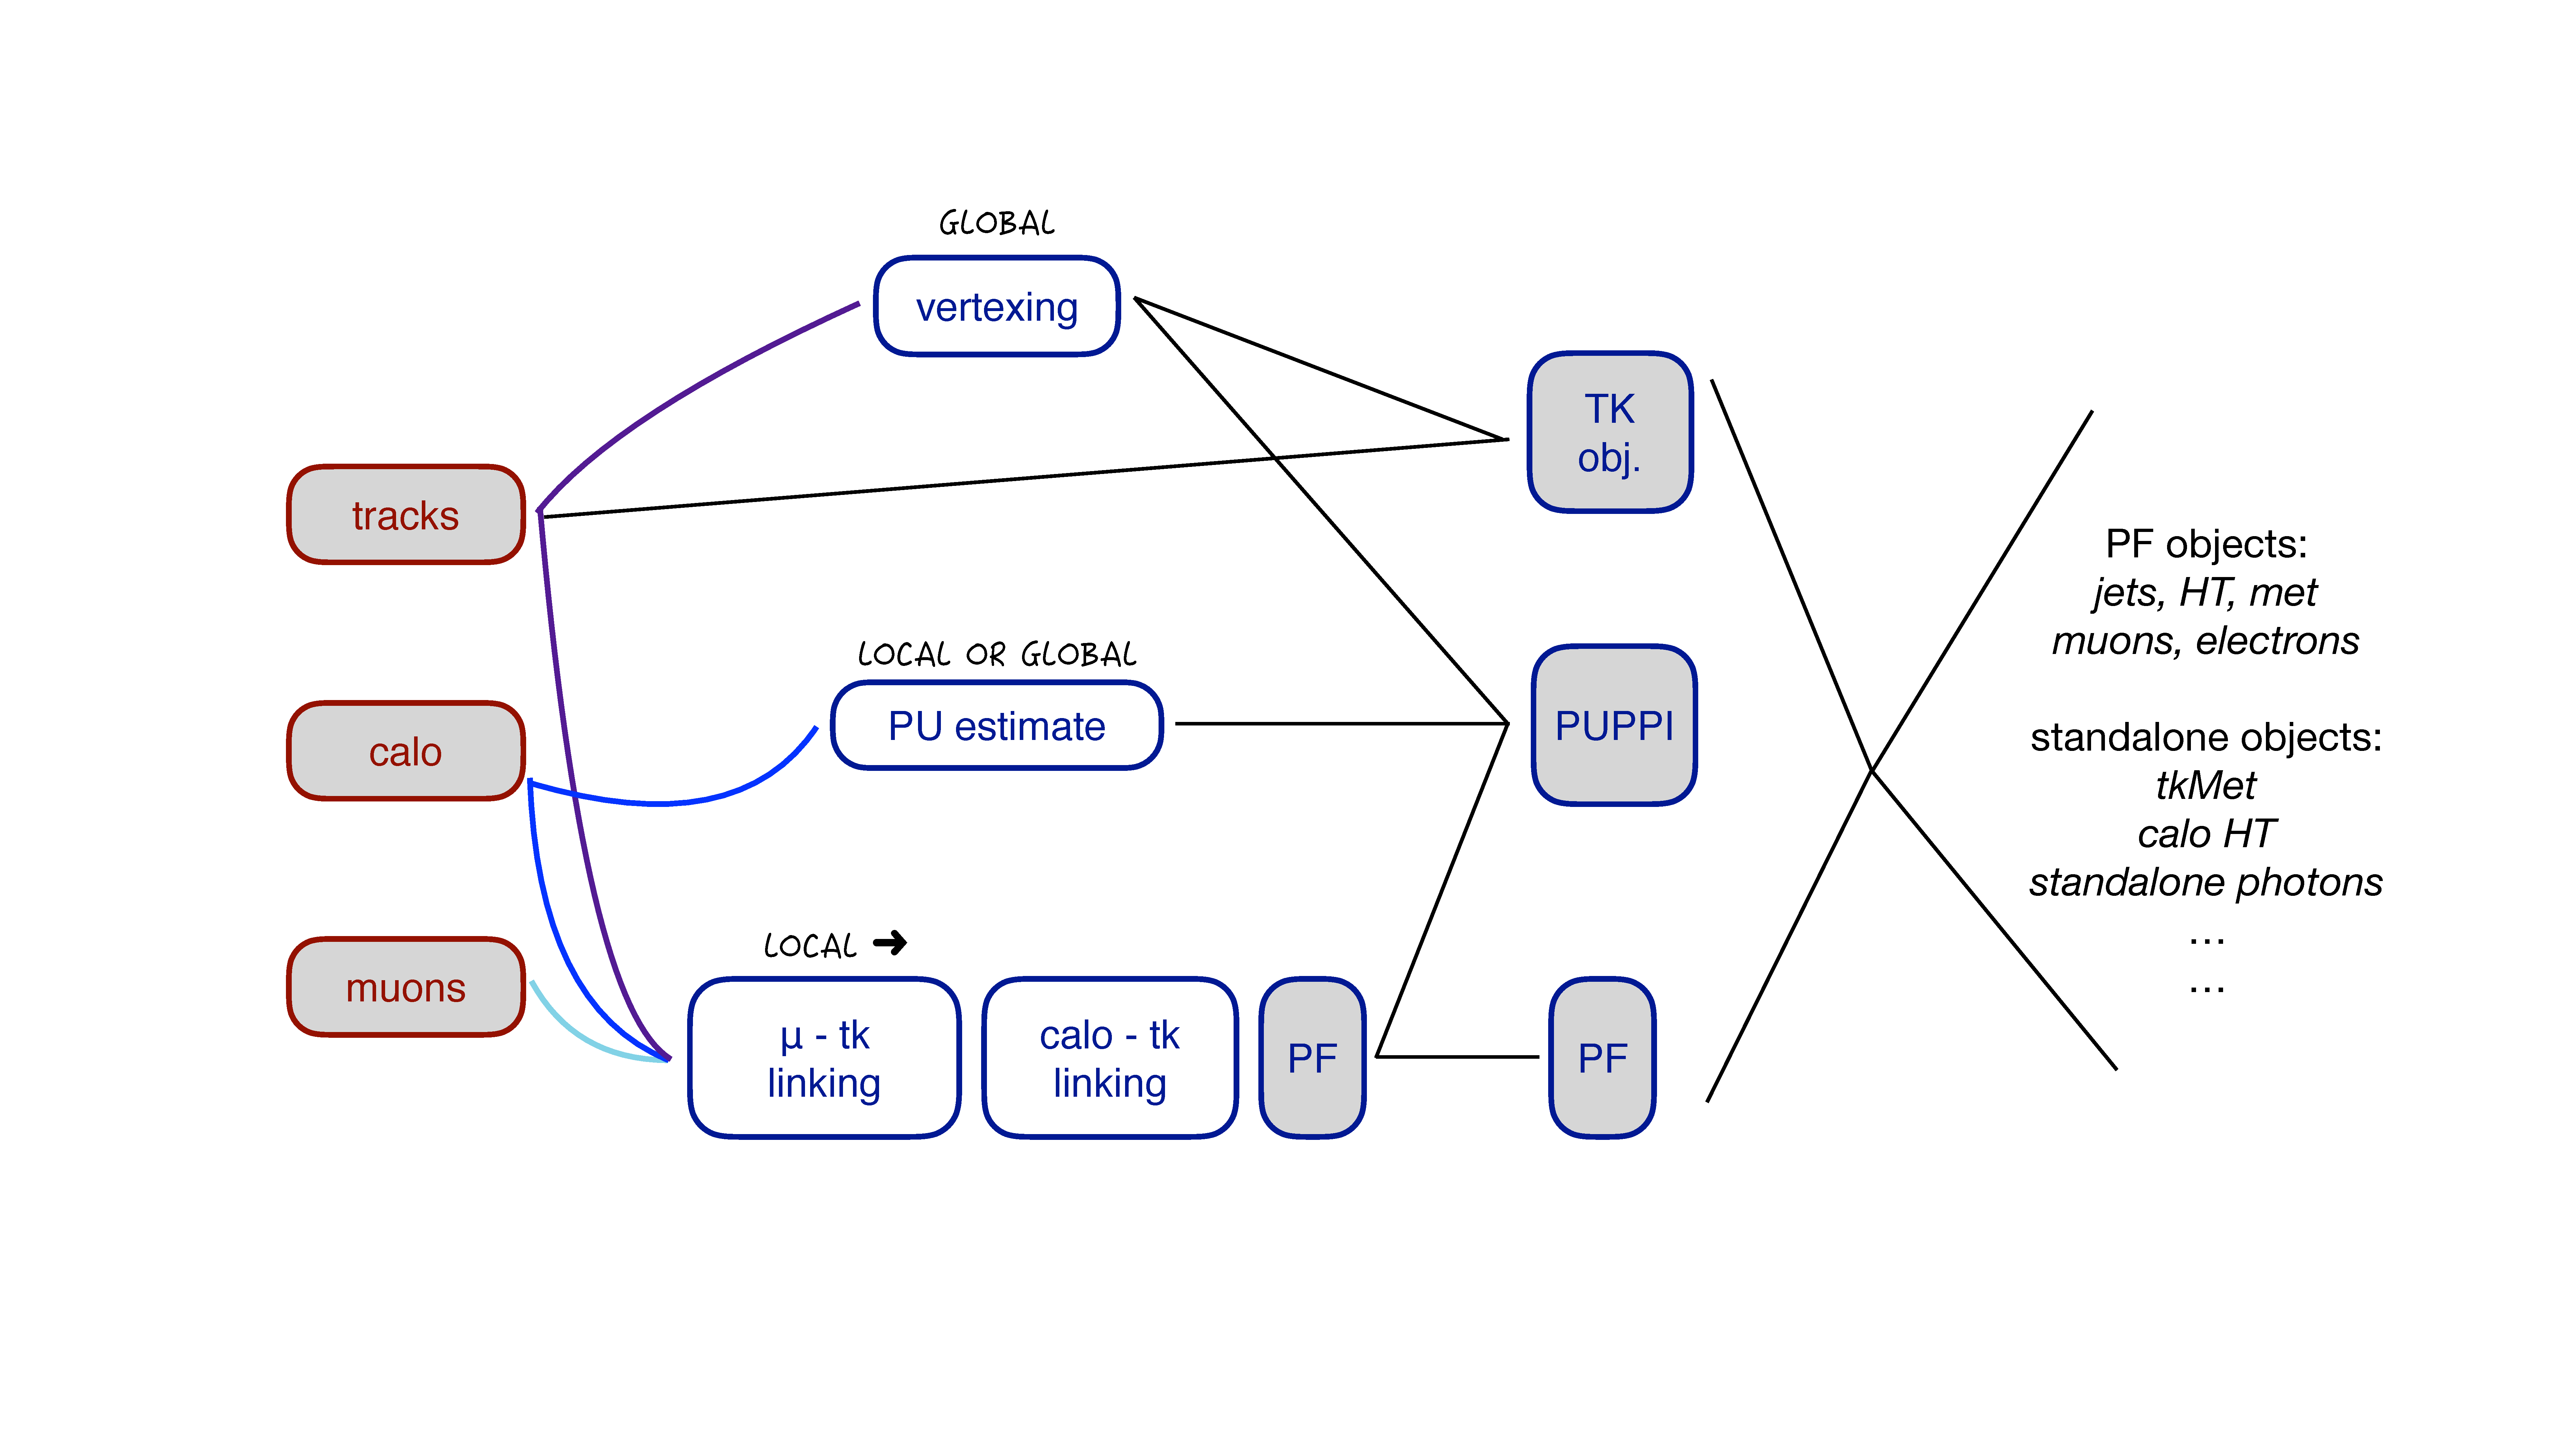
\includegraphics[width=0.9\textwidth] {figures/l1pfp.pdf}
\caption{
Overview of the L1PFP algorithm
\label{fig:l1pfp}
}
\end{figure}

The local operation steps proceed in the following order: 
\begin{enumerate}
\item Track-muon linking: combines muon tracks and tracker tracks to make muon objects
\item Track-calo linking: links calorimeters cells with tracker tracks to define both charged and neutral hadrons and photons and electrons
\item PUPPI: performed in parallel to the vertexing and pileup estimate, estimates the likelihood of being pileup
\end{enumerate}

Each of these, as well as the global operations, are described in further detail below.  
After the computation of the L1PFP particle candidates, the physics objects can be computed such as jets, MET and lepton information.  
It should be noted other standalone objects may also be computed at this stage such as track-based MET and calorimeter based photons.

\subsubsection{Vertexing and pileup estimate}

Vertexing is an extremely important step in the pileup mitigation of any algorithm. 
Pileup interactions occur at different points in the beam spot and differentiating each interaction's z position helps to reject uninteresting pileup interactions. 
We currently follow the histogramming algorithm proposed in~\cite{Contardo:2020886} to do a fast vertexing using the track trigger tracks.
The method bins the tracks in their Z vertex position.  
We bin the tracks from $\delta z = ( -20\cm,20\cm )$ with a bin size of 1.3\mm summing the bin content by track $\pt_{tk}'$ where $\pt_{tk}'$ = $\text{min}(50\GeV, \pt^{tk})$ 
and $\pt^{tk}$ is the track \pt.
We do not allow the track \pt to be greater than 50\GeV in order to minimize the effect from fake tracks.
The primary vertex $\delta z$ is labeled $\delta z_{PV}$ and is defined as the center of the bin with the largest $\Sigma \pt_{tk}'$.
We then define tracks from the primary vertex as tracks within $\delta z_{PV} = \pm 1.95~\mm$

{\color{red} to do: make a few plots to demonstrate vertexing efficiency}



\subsubsection{Track-Muon linking}
\subsubsection{Track-Calo linking}
\subsubsection{Regional definitions}
\subsubsection{Integer emulation}